%%%%%%%%%%%%%%%%%%%%%%%%%%%%%%%%%%%%%%%%%%%%%%%%%%%%%%%%%%%%%%%%%%%%%%%%%%%%%%%%%%%%%%%%%%%
%%%%%%%%%%%%%%%% INTRODUCCION Y CONTEXTO  ABC %%%%%%%%%%%%%%%%%%%%%%%%%%%%%%%%%%%%%%%
%%%%%%%%%%%%%%%%%%%%%%%%%%%%%%%%%%%%%%%%%%%%%%%%%%%%%%%%%%%%%%%%%%%%%%%%%%%%%%%%%%%%%%%%%%%
\chapter{Contexto de los Sistemas ABC}\label{ch:introSistemasABC}

%%%%%%%%%%%%%%%%%%%%%%%%%%%%%%%%%%%%%%%%%%%%%%%%%%%%%%%%%%%%%%%%%%%%%%%%%%%%%%%%%%%%%%%%%%%
%%%%%%%%%%%%%%%%%%%%%%%%%%%%%%%%%%%%%%% SISTEMAS ABC %%%%%%%%%%%%%%%%%%%%%%%%%%%%%%%%%%%%%%%
%%%%%%%%%%%%%%%%%%%%%%%%%%%%%%%%%%%%%%%%%%%%%%%%%%%%%%%%%%%%%%%%%%%%%%%%%%%%%%%%%%%%%%%%%%%
\section{Sistemas ABC}\label{sec:sistemasABC}

\subsection{Definición}

\begin{figure}
    \centering
    \includegraphics[width=0.8\textwidth]{ch-sistemasABC/images/ch-SistemasABC/ABCsEnElAeropuertoPortugal.png}
    \caption{Sistemas \gls{ABC} en el aeropuerto Humberto Delgado (Liboa, Portugal) \cite{ABC4EUOnline}}
    \label{fig:ABCEnElAeropuerto}
\end{figure}

Las acciones y las comprobaciones que deben realizarse en un control de frontera para autorizar el cruce de un viajero, dependen del tipo de frontera, de los países de origen y de destino, y del propio viajero. Pero, básicamente se resumen en cuatro operaciones que los agentes de frontera en primera linea\footnote{Se conoce como primera linea al área dentro de los puntos de cruce de frontera donde se sitúan los agentes para realizar los controles pertinentes.}, deben realizar, en el menor tiempo posible: 

\begin{itemize}
    \item
    Verificar la autenticidad de la documentación del viajero.
    \item
    Verificar la identidad del viajero contra la identidad almacenada en los documentos que porta.
    \item
    Chequear la autorización del viajero para cruzar la frontera y comprobar que cumple las condiciones de entrada entrada en el país. 
    \item
    Analizar las posibles amenazas de seguridad.
\end{itemize} 

El flujo de viajeros ha ido creciendo constantemente durante los últimos años y la \textit{International Air Transport Association} (\GLS{IATA} \cite{IATAOnline}) estima que para $2025$ habrá unos $887$ millones de viajeros en Europa y $7$ mil millones para $2034$, en todo el mundo \cite{IATA/REVIEW/2016}. Este incremento de viajeros y el uso de nuevas tecnologías para la falsificación de documentos y para la \textit{suplantación de identidades}, deja claro que un enfoque únicamente manual no es suficiente y resulta necesario el uso de sistemas automáticos, como los \textit{Automated Border Control} \GLS{ABC} que complementen el trabajo de los agentes.

Los sistemas \GLS{ABC} son sistemas automáticos o semiautomáticos para la identificación de viajeros en los cruces de frontera. Se basan en la lectura automática de los documentos de viaje y en la verificación biométrica. Deben realizar las mismas comprobaciones en un tiempo igual o menor al de los procesos manuales, permitiendo de este modo: facilitar los cruces, aumentar el flujo de viajeros y mantener los estándares de seguridad, sin necesidad de incrementar el número de guardias de seguridad.

Actualmente, la mayoría de los aeropuertos internacionales disponen de sistemas \GLS{ABC} en sus cruces de frontera (ver Fig. \ref{fig:MapaABCMudialesIATA} ), y también, cada vez es más frecuente encontrar estos sistemas en otro tipo de fronteras, como puertos marítimos o fronteras terrestres (ver Fig. \ref{fig:fronterasConABC}). 

\begin{figure}
    \centering
    \includegraphics[width=0.7\textwidth]{ch-sistemasABC/images/ch-SistemasABC/ABC_TipoFronteras.png}
    \caption{Sistemas \GLS{ABC} por tipos de fronteras.}
    \label{fig:fronterasConABC}
\end{figure}

\begin{figure}
    \centering
    \includegraphics[width=0.8\textwidth]{ch-sistemasABC/images/ch-SistemasABC/AeropuertosConSistemasABCMapaIATA.png}
    \caption{Aeropuertos internacionales con distintos tipos de sistemas \GLS{ABC} en $2019$. \textit{International Air Transport Association} (\GLS{IATA} \cite{IATAOnline}).}
    \label{fig:MapaABCMudialesIATA}
\end{figure}


%%%%%%%%%%%%%%%%%%%%%%%%%%%%%%%%%%%% SISTEMAS ABC:FUNCIONAMIENTO DE LOS SISTEMAS ABC %%%%%%%%%%%%%%%%%%%%%%%%%%%%%%%%%%%%
\subsection{Funcionamiento}\label{sec:funcionamientoABC}

Las tareas fundamentales a realizar en un cruce de fronteras con sistemas automáticos consisten en: El escaneo del pasaporte, la autenticación de la documentación de viajero, la comprobación de su idoneidad para cruzar la frontera y la verificación de su información biométrica. Además de éstas, existen otras tareas no automáticas y una tarea fundamental que involucra a todas las demás que es controlar la seguridad de todo el proceso.

\begin{itemize}
    \item 
    \textbf{Escaneo del pasaporte} 
    
    El viajero debe portar un \textit{Electronic machine-readable travel document} (\gls{eMRTD}), legible por el sistema y que cumpla con las especificaciones dadas para este tipo de documentos por la \textit{International Civil Aviation Organization} (\GLS{ICAO} \cite{ICAOOnline}) en el informe \GLS{ICAO} Doc $9303$ \cite{doc20069303}. El \gls{eMRTD}, habitualmente un \textit{Electronic Passport} \gls{e-passport}, debe incluir la información biométrica del viajero portador \footnote{Para más información sobre los documentos de viaje es posible consultar en \GLS{ICAO}-Doc $9303$ \cite{doc20069303} y el Apéndice \ref{apendix:DocDeViaje} donde se detallan los documentos soportados por los sistemas \GLS{ABC}.}.
    
    El viajero debe colocar el documento de viaje, en el lector de documentos por la hoja de datos de forma que quede visible la \textit{Machine-Readable Zone} (\GLS{MRZ}, Figura \ref{fig:HojaDatos_MRZ} b)). 
    
    En caso de que el viajero no porte documentación valida o ésta no pueda ser leída, el viajero será rechazado.
    
    \item
    \textbf{Autenticación y verificación de la documentación}
    
    Tras escanear el documento es necesario comprobar su \textbf{autenticidad} y confirmar que sean \textbf{documentos válidos y genuinos}. 
    
    Con la imagen capturada del documento se realiza un proceso de lectura automático \textit{Optical Character Recognition} (\GLS{OCR}) sobre la \GLS{MRZ}, donde se leen algunos datos biográficos del viajero. Y de forma simultanea, mediante radio-frecuencia se extrae la información almacenada en el chip \GLS{RFID} integrado en el documento \gls{eMRTD}. 
    
    Para autenticar los documentos, la información visual leída se contrasta con la extraída del chip.

    Además de autenticar la identidad de la documentación, también se examinan las medidas de seguridad y de antifalsificación que tienen los pasaportes (para ver algunas de estas medidas ver la Figura \ref{fig:MarcasSeguridadDocumentos}, en el Apéndice  \ref{apendix:DocDeViaje}).
    
    \item
    \textbf{Comprobación de la información biométrica}
    
    Se realiza una verificación de la identidad del viajero mediante sus datos biométricos. Dependiendo de los sistemas y del tipo de documentación se pueden usar unos rasgos biométricos u otros. Los rasgos que más comúnmente se capturan en los sistemas \GLS{ABC} son la cara, para biometría \gls{facial}, huellas dactilares en la biometría \gls{dactilar} o los ojos en la \textbf{biometría del \gls{iris}}. (Por ejemplo, el sistema puede capturar una imagen en vivo de la cara del viajero y compararla con la cara impresa en el pasaporte o con la almacenada en el chip).
    
    \item
    \textbf{Idoneidad del viajero}
    
    Además de controlar la autenticidad de los documentos y la identidad del viajero, también se debe comprobar la elegibilidad y la autorización del viajero para cruzar la frontera. Esto depende del viajero en sí y de las reglas y los requisitos de cada país.  
    Para decidir si el viajero es apto o no para cruzar la frontera se requiere consultar bases de datos y registros centrales a los que los sistemas \GLS{ABC} deben tener acceso, como : \textit{Schengen Information System} (\textbf{\GLS{SIS}}) en las fronteras de \GLS{EU}; \textit{Visa Information System} (\textbf{\GLS{VIS}}), para el control de visados; National \GLS{PKD}, con los encriptados del chip, especificos en cada pais; \textit{Vehicle Registration Certificate} (\GLS{VRC}), en algunas fronteras terrestres; \GLS{AFIS-ABIS}, para el registro de huellas dactilares; etc. % \Gls{INTERPOL}, \textit{Opt.national}.

    \item
    \textbf{Tareas no automatizadas}
    
    En algunos casos, para determinados viajeros, los controles automáticos de los \GLS{ABC} no son son suficientes y se requieren otros procesos que por ahora se deben realizar manualmente como por ejemplo, el estampado del pasaporte o alguna de las comprobaciones del visado (entrevista de los agentes de seguridad). 

    \item
    \textbf{Seguridad}
    
    Los sistemas deben de garantizar la seguridad en todos los procesos y sólo en el caso de que todos procesos del sistema \GLS{ABC} se realicen de forma satisfactoria el viajero podrá cruzar la frontera. Si se produce algún fallo los agentes de seguridad que controlan los sistemas de forma remota, se harán cargo de la situación. También en el caso de que algún viajero no pueda usar los sistemas automáticos debe ser dirigido a los controles manuales.

\end{itemize}


%%%%%%%%%%%%%%%%%%%%%%%%%%%%%%%%%%%% SISTEMAS ABC:ARQUITECTURA %%%%%%%%%%%%%%%%%%%%%%%%%%%%%%%%%%%%
\subsection{Arquitectura}\label{sec:AquitecturaABC}

\begin{figure}
    \centering
    \includegraphics[width=1\textwidth]{ch-sistemasABC/images/ch-SistemasABC/ArquitecturaEnAeropuerto.png}
    \caption{Esquema aeropuerto con sistemas \GLS{ABC}s \cite{labati2016biometric}.}
    \label{fig:EsquemaAeropuerto}
\end{figure}


Los sistemas \GLS{ABC} tienen una arquitectura física y una arquitectura lógica. Cada \GLS{ABC} esta compuesto por uno o varios dispositivos que son su arquitectura física, sobre la que se implementan las tareas de un conjunto de subsistemas que interactuaban entre si y que integran la arquitectura lógica del sistema.

Dependiendo de como se distribuya la arquitectura lógica en los dispositivos físicos, se distinguen distintos tipo de \textbf{topologías de sistemas \GLS{ABC}}.


%%%%%%%%%%%%%%%%%%%%%%%%%%%%%%%%%%%% SISTEMAS ABC:ARQUITECTURA LOGICA %%%%%%%%%%%%%%%%%%%%%%%%%%%%%%%%%%%%
\subsubsection{Arquitectura lógica}\label{subsec:ArquitecturaLogicaABC}

\begin{figure}
    \centering
    \includegraphics[width=0.7\textwidth]{ch-sistemasABC/images/ch-SistemasABC/SUBSISTEMAS_ABC.png}
    \caption{Subsistemas y servicios externos de de un sistema \GLS{ABC} \cite{labati2016biometric}.}
    \label{fig:SubsistemasABC}
\end{figure}

La arquitectura lógica de los sistemas se encarga de la realización de dos procesos principales: \textit{Register Traveller Program} (\textbf{\GLS{RTP}}) y \textit{Entry/Exit System} (\textbf{\GLS{EES}}). Y para ello cuenta con una serie de \textbf{subsistemas} que además de comunicarse entre ellos, interactúan con una serie de \textbf{servicios externos} (ver Fig. \ref{fig:SubsistemasABC}).

Para garantizar una correcta comunicación entre los distintos módulos y con los sistemas externos, es necesario que los \GLS{ABC} sigan una serie de especificaciones en sus protocolos de comunicación, interfaces y formatos de intercambio \footnote{\GLS{ISO}/\GLS{IEC} 19794, define un estándar para el intercambio de información entre los distintos módulos de un sistema biométrico.}.
    
Seguir estos estándares también permite una mayor flexibilidad y modularidad en los sistemas, ya que permite modificar un modulo del sistema sin cambiar el sistema completo.

\medskip
\textbf{Procesos}

Existen distintos protocolos, dependiendo del tipo de viajero, del país de origen, del tiempo de estancia en país de destino, etc. Pero los procesos comunes a todos los \GLS{ABC} son: \GLS{RTP} y \GLS{EES}. 

\begin{itemize}
    \item 
    \textbf{\GLS{RTP}}
    
    Se verifica la identidad del viajero y su adecuación para cruzar la frontera atendiendo a la información almacenada en su documentación. Este proceso puede realizarse de forma previa al viaje, en el caso de viajeros frecuentes o registrados con anterioridad, o bien ya en el aeropuerto, normalmente en dispositivos \gls{e-kiosk}. La información biométrica del viajero, capturada en el momento (\gls{vivo}) se verifica con la almacenada en sus documentos de viaje.
    
    \item 
    \textbf{\GLS{EES}}
    
    Este proceso se realiza en dispositivos \gls{e-gate}, ya en el cruce de fronteras.
    Y consiste en el emparejamiento entre el la información biométrica registrada y los datos capturados \textit{in-vivo} de viejo en el momento del cruce. Es decir, la información biométrica es nuevamente capturadas y se compara con la capturada en el proceso \GLS{RTP}.
\end{itemize}

\medskip
\textbf{Subsistemas}

Para la realización de los procesos \GLS{RTP} y \GLS{EES} intervienen una serie de subsistemas dentro del sistema \GLS{ABC}:

\begin{itemize}
    \item 
    \textbf{DAS} (\textit{Document Authentication System}): Evalúa la validez y la legitimidad de la documentación del viajero. Además de verificar las marcas de autenticidad de los documentos, lee la zona legible del documento \GLS{MRZ} y la información almacenada en el chip en caso de que sea un \gls{eMRTD}. 
    
    \item 
    \textbf{\GLS{BVS}} (\textit{Biometric Verification System}): Se encarga de verificar la información biométrica del viajero capturada en el sistema (\gls{vivo}), con la leída en la documentación. 
    
    \item 
    \textbf{CSI} (\textit{Control System Interface}): Gestiona la comunicación con las interfaces externas. Por ejemplo, para comprobar la idoneidad del viajero. Dependiendo de la normativa de cada país los \GLS{ABC} se conectan a unos servicios u a otros. 
    
    \item
    \textbf{BGMS} (\textit{Border Guard Maintenance System}): Incluye las tareas de control y de monitorización de los agentes de frontera. 
\end{itemize}

\textbf{Servicios externos}

\begin{itemize}
    \item 
    \textbf{VMS} (\textit{Visa Management System}): 
    
    Se encarga de las gestiones con el sistema \GLS{VIS} (\textit{Visa Information System}).
    
    Base de datos con el toda la información sobre el visado del viajero\footnote{El parlamento europeo en $2008$ definió la información del sistema \GLS{VIS} para todos los países de la Unión:  https://eur-lex.europa.eu/legal-content/EN/TXT/?uri=CELEX\%3A32008R0767.} : Tipo de visado, información personal del viajero, biométrica y biográfica, información del viaje, fecha de entrada, duración del visado.
    
    Los sistemas \GLS{ABC} se comunican con este sistema mediante el número de visa, un número identificador y los datos biométricos del viajero.

    \item 
    \textbf{RTP} (\textit{Registered Traveller Programme}).
    
    Base de datos con la información ciertos viajeros que se han registrado previamente en sistema\footnote{La Unión Europea está analizando este tipo de pre-registro para si fronteras. Diferentes proyectos en el marco FP$7$, como \GLS{ABC4EU} o \GLS{FastPass}, estudian este tipo de procesos.}. El registro previo es voluntario y simplifica un posterior cruce de fronteras, mejorando la seguridad y reduciendo el tiempo del proceso. 
    
    El registro previo está pensado para viajero que por razones laborales o familiares viajan frecuentemente a un determinado país.
    
    El proceso de \GLS{RTP} involucra la captura de la información biométrica del viajero.   
    
    
    \item 
    \textbf{EEMS} (\textit{Entry/Exit Management System}):
    
    Se encarga de las gestiones con el sistema \GLS{EES} (\textit{Entry/Exit System}).
    
    Base de datos que almacena la información del los viajero que cruzan el cruce de fronteras.
    
    Rechaza el antiguo estampado del sello en los documentos.
    
    Almacena información biométrica del viajero.
    
    Permite comprobar a los agentes si lo viajeros han sobrepasado el tiempo de estancia en el país.
    
    Permite a las naciones controlar el flujo de migrantes.
    
    \item 
    \textbf{\GLS{SIS}} (\textit{Schengen Information System}):
    
    Sistema especifico para los viajeros de la Unión Europea (\GLS{EU}). Contienen datos biométricos, como la cara o las huellas dactilares. También contiene información de las agencias de seguridad europeas sobre personas vulnerables y personas peligrosas.  
    
    \item 
    \textbf{\GLS{ETIAS}} (\textit{European Travel Information and Authorisation System}):
    
    Sistema especifico de pre-registro para \GLS{TCNVE} en el área \Gls{Schengen}. Aprobada por la en en $2018$ y comienza a ser operativa en $2022$ \cite{union2018directiveETIAS}.
    
    \item 
    \textbf{\GLS{FADO}} (\textit{False and Authentic Documents Online}):
    
    Base de datos con el formato de los pasaportes originales de cada país e información sobre tipos de falsificaciones en documentos de viaje.
    
\end{itemize}

%%%%%%%%%%%%%%%%%%%%%%%%%%%%%%%%%%%% SISTEMAS ABC:ARQUITECTURA FISICA %%%%%%%%%%%%%%%%%%%%%%%%%%%%%%%%%%%%
\subsubsection{Arquitectura física}\label{subsec:ArquitecturaFisicaABC}

Los sistemas \GLS{ABC} pueden estar compuestos de varios dispositivos y sensores con los que el viajero interactúa para realizar los distintos los procesos (ver Fig. \ref{fig:ElementosFisicosABC}). Dentro de estos dispositivos se pueden encontrar:

\begin{figure}
    \centering
    \includegraphics[width=1\textwidth]{ch-sistemasABC/images/ch-SistemasABC/ELEMENTOS_FISICOS_SISTEMAS_ABC.png}
    \caption{Componentes físicos más comunes de los dispositivo \GLS{ABC} (\GLS{ICAO}\cite{ICAOOnline})}
    \label{fig:ElementosFisicosABC}
\end{figure}

\begin{itemize}
\item 
\textbf{Barreras físicas}, que pueden ser una o varias.

\item
\textbf{Lector de documentos}, preparado para la lectura óptica de los documentos y para la lectura por radiofrecuencia de chip en el caso de documentos \gls{eMRTD}.

\item
\textbf{Dispositivos de captura biométrica}: Cámaras, lectores de huellas dactilares u otro tipo de sensores.

\item
\textbf{Dispositivos para la interacción con el usuario}: Monitores, botones, señales luminosas o altavoces.

\item
\textbf{Sistemas de proceso} donde se ejecuten las distintas tareas. 

\item
\textbf{Sistemas de comunicaciones}: Controladores, conexiones, hubs, etc.

\item
\textbf{Sensores y cámaras de vigilancia} para el correcto funcionamiento del sistema: Detectar objetos abandonados, circuitos de videovigilancia o detectar varios viajeros dentro del dispositivo, etc.  

\item
Una \textbf{estación de control} para que los operadores monitoricen y gestionen de forma remota los sistemas .
\end{itemize}

Para lo sistemas que están instalados en el exterior también deben considerarse elementos para proteger los sistemas de las condiciones climáticas y de actos vandálicos: Puertas protectoras, cerraduras, fijaciones, etc.


%%%%%%%%%%%%%%%%%%%%%%%%%%%%%%%% SISTEMAS ABC:TOPOLOGIAS DE ABC %%%%%%%%%%%%%%%%%%%%%%%%%%%%%%%%%%%%%%%%%
\subsubsection{Topologías}\label{subsec:Topologias}

Dependiendo de la disposición de los dispositivos físicos y de las tareas que se realizan en cada dispositivo se pueden considerar distintas topologías de sistemas \GLS{ABC}.

Si la validación de los documentos y la verificación de la identidad del viajero, se realizan en un único proceso el sistema tiene una topología \textit{<<One Step>>}, mientras que si esas tareas se desdoblan en los dos procesos (\GLS{RTP} y \GLS{EES}) tendrá una topología \textit{<<Two Step>>}. Los sistemas \GLS{ABC} con topología de dos pasos puede tratarse a su vez, de una topología \textit{<<Integrated Two Step>>} o \textit{<<Segregated Two Step>>}.    

\begin{figure}
    \centering
    \includegraphics[width=0.8\textwidth]{ch-sistemasABC/images/ch-SistemasABC/topologiasABC.png}
    \caption{(a). Topología \GLS{ABC} \textit{<<One Step>>}. (b). Topología \GLS{ABC} \textit{<<Integrated Two Step>>}. (c). Topología \GLS{ABC} \textit{<<Segregated Two Step>>}. \cite{FRONTEX2016OpeReport}}
    \label{fig:TopologiasABC}
\end{figure}

\medskip
\textbf{Topología \textit{<<One Step>>}}
\medskip

En la topología \textit{<<One Step>>} los procesos de \GLS{RTP} y \GLS{EES} se fusionan en un único proceso en el que se realiza la identificación del viajero en el mismo momento en el que éste cruza la frontera (Figura \ref{fig:TopologiasABC} (a)). Verificación y seguridad se realizan en una única transición. 

Los dispositivos con este tipo de topologías suelen ser \gls{e-gate} de tipo \gls{mantrap} (Figura \ref{fig:dispositivosABCEstaticos} b)) que no permiten el paso hasta que no se ha realizado correctamente la identificación. Aun así  son más rápidos ya que pueden realizar algunas acciones en paralelo. Por ejemplo, capturar los datos biométricos del viajero mientras se consulta su elegibilidad con los datos biográficos.

\medskip
\textbf{Topología \textit{<<Two Step>>}}
\medskip

En las topologías \textit{Two Steps} los procesos \GLS{RTP} y \GLS{EES} están bien diferenciados. Primero el viajero es registrado y a continuación se verifica su información biométrica antes de permitir el cruce. 

Dependiendo de si los procesos se realizan en un mismo dispositivo o en dos, se distingue entre topologías \textit{<<Integrated Two Steps>>} (Figura \ref{fig:TopologiasABC} (a)) y \textit{<<Segregated Two Step>>} (Figura \ref{fig:TopologiasABC} (b)).

\begin{itemize}
    \item 
    \textbf{Topología \textit{<<Integrated Two Step>>}}
    
    La verificación de documentación y la comprobación de la idoneidad del viajero se realiza en una etapa, necesaria para proceder a una segunda etapa en la que se realiza la verificación biométrica y otras operaciones de control.
    
    Los procesos de \GLS{RTP} y \GLS{EES} se realizan en el mismo dispositivo, habitualmente un \gls{mantrap}, como en las topologías \textit{<<One Step>>}
    
    \item
    \textbf{Topología \textit{<<Segregated Two Step>>}}
    
    El proceso \GLS{RTP} se realiza en un dispositivo, habitualmente un \gls{e-kiosk} (Figura \ref{fig:dispositivosABCEstaticos} (a)) y el \GLS{EES} en otro dispositivo distinto una \gls{e-gate} (Figura \ref{fig:dispositivosABCEstaticos} (c)).    
    
    Una primera etapa en la que se realiza la verificación del viajero y la captura de los datos biométricos del viajero, que generan un \textit{\gls{token}} \footnote{Alguna publicaciones llaman a esta biometría pre-pregistrada \gls{biometria} <<táctica>>.} con el cual, en una segunda etapa, se realizará una nueva verificación, con los datos del viajero que desea cruzar la frontera.

    Los sistemas segregados permiten optimizar el espacio y el tiempo respecto de las topologías con procesos integrados, pero también pueden confundir a los viajero inexpertos que pueden no entender claramente por que el proceso esta dividido en dos pasos. También requiere más mantenimiento al tratarse de dos dispositivos.
\end{itemize}

%%%%%%%%%%%%%%%%%%%%%%%%%%%%%%%%%%% SISTEMAS ABC:TIPOS DE ABC %%%%%%%%%%%%%%%%%%%%%%%%%%%%%%%%%%%%%%%%%
\subsection{Tipos de sistemas}\label{sec:tiposABC}

\begin{figure}
 \centering
     \includegraphics[width=0.8\textwidth]{ch-sistemasABC/images/ch-SistemasABC/CATERGORIAS_DE_ABCS.png}     \caption{Categorías de los sistemas \GLS{ABC} atendiendo a distintos aspectos.}
    \label{fig:categoriasABC}
\end{figure}


Los sistemas \GLS{ABC} se pueden clasificar atendiendo a distintas características (Ver Fig. \ref{fig:categoriasABC}): Atendiendo al grado de autonomía del viajero, al tipo de identificación, al tipo de documentos capaz de procesar, a su topología o atendiendo al tipo de dispositivos de adquisición.

\begin{itemize}
%%%%%%%%%%%%%%%%%% SISTEMAS ABC:POR AUTONOMIA 
\item
Tipos de \GLS{ABC} \textbf{atendiendo a su autonomía}

Los sistemas \GLS{ABC} pueden ser automáticos o semiautomáticos \footnote{Los sistemas automáticos también se conocen como desatendidos y a los semiautomáticos como atendidos.}, dependiendo de si el viajero puede realizar todos los procesos de manera automática sin requerir ningún tipo de asistencia por parte de los agentes de seguridad. (Que un agente sea requerido para subsanar una incidencia no hace que el sistema deje de ser considerado como automático).

%%%%%%%%%%%%%%%%%% SISTEMAS ABC:POR MODO DE IDENTIFICADION
\item
Tipos de \GLS{ABC} \textbf{atendiendo al modo de identificación}

Dependiendo de si el sistema requiere un \textit{\gls{token}} para identificar al viajero se distinguen dos tipos de sistemas: \textbf{\textit{\gls{token-required}}} o \textbf{\textit{\gls{tokenless}}} \cite{ISO/Biometric}.

\begin{itemize}
    \item
    \textit{\textbf{\gls{token-required}}}:
    Requieren de un \textit{\gls{token}}, para realizar la identificación del viajero, que bien puede ser un \textit{\gls{token} físico}, como el propio \gls{e-passport} u otro \gls{eMRTD}, o bien un \textbf{\textit{\gls{token}} lógico} que puede ser una \textbf{clave} o un rasgo biométrico pre-registrado\footnote{Algunas publicaciones consideran los sistemas que usan \gls{biometria} pre-registrada como \gls{tokenless}.}.
    \item
    \textit{\textbf{\gls{tokenless}}}:
    No requieren de un \textit{\gls{token}} para realizar la identificación del viajero. El viajero puede presentar un rasgo biométrico al sistema y éste realiza una búsqueda \textbf{$(1:n)$} con todos los usuarios del sistema.
\end{itemize}

Normalmente los cruces de frontera requieren que los viajeros porten algún documento identificativo por lo que la mayoría de los sistemas \GLS{ABC} instalados en cruces de frontera son \GLS{ABC} \textit{\gls{token-required}}.

%%%%%%%%%%%%%%%%%% SISTEMAS ABC:POR DOCUMENTOS QUE PROCESAN
\item
Tipos de ABC \textbf{atendiendo a los documentos que procesan}

Los sistemas \GLS{ABC} pueden clasificarse dependiendo de los documentos que puede procesar: \gls{e-passport}, \gls{nacional-ID}\footnote{Algunos países de la \GLS{EU}, como España o Alemania disponen de documentos de identificación  \gls{eID}, con información biométrica del propietario y que son válidos para el cruce de fronteras.}, \Gls{visa}\footnote{En la \GLS{EU} el documento \GLS{visa} es un documento de viaje obligatorio en para muchos países fuera del acuerdo \gls{Schengen}.}. 

%%%%%%%%%%%%%%%%%% SISTEMAS ABC:POR TOPOLOGIA
\item
Tipos de \GLS{ABC} \textbf{atendiendo a su topología}

Los sistemas \GLS{ABC} dependiendo del número de dispositivos y de los procesos que se realizan en cada uno de ellos se distinguen sistemas \GLS{ABC} \textit{<<One Step>>}, \textit{<<Integrated Two Step>>}, o \textit{<<Segregated Two Step>>}. (En las Sección \ref{subsec:Topologias} se explica en detalle cada una de las topologías). 

%%%%%%%%%%%%%%%%%% SISTEMAS ABC:POR DISPOSITIVOS DE ADQUISICION
\begin{figure}
 \centering
     \includegraphics[width=0.8\textwidth]{ch-sistemasABC/images/ch-SistemasABC/dispositivosABCEstaticos.png}
     \caption{(a) \gls{e-kiosk}, (b) \textit{e-gate mantrap} y (c) \gls{e-gate} con una barrera.}
    \label{fig:dispositivosABCEstaticos}
\end{figure}

\item
Tipos de \GLS{ABC} \textbf{atendiendo a los dispositivos de adquisición}

Dependiendo de los dispositivos en los que se implementa el sistema, Un \GLS{ABC} puede ser: \GLS{ABC} estáticos cuando los dispositivos no pueden desplazarse (Figura \ref{fig:dispositivosABCEstaticos}) y es el viajero quien debe aproximase al dispositivos para ser identificado y \GLS{ABC} móviles, cuando el sistema se ha implementado en un dispositivos móviles (por ejemplo una \textit{tablet}) y es el agente quien se aproxima al viajero para realizar la identificación.

\medskip
\textbf{\GLS{ABC} estáticos}

Dentro de los dispositivos estáticos, se pueden distinguir un nuevo tipo sistemas que son los Sistemas \GLS{ABC} estáticos con captura \gls{OnTheFly} o sistemas \GLS{ABC} \gls{OnTheFly} (Descritos en detalle en el capitulo \ref{ch:ABC_OnTheFly}) que se diferencian de los sistemas \GLS{ABC} con captura estática en que no requieren que el viajero se detenga frente al dispositivo.  

\medskip
\textbf{\GLS{ABC} móviles}

Fronteras exteriores donde se requiere una identificación pero no es posible el uso de \glspl{e-gate}, como por ejemplo cruces de fronteras en autobuses, coches o trenes.

Los sistemas móviles son útiles también, como sistemas adicionales y de apoyo a para los agentes en las puertas \GLS{ABC}.

Los requisitos básicos a los que deben atender los sistemas \GLS{ABC} móviles son:

\begin{itemize}
\item
\Gls{captura} de datos biométricos de forma cómoda y confiable.

\item
Seguridad en las comunicaciones inalámbricas.

\item
Dispositivos móviles adaptados al trabajo de los agentes de seguridad: \Gls{usabilidad}, duración de las baterías, robustez, \textit{Human-Machine Interface} (\textbf{\GLS{HMI}}).

\end{itemize}

\end{itemize}



%%%%%%%%%%%%%%%%%%%%%%%%%%%%%%%%%%%%%%%%%%%%%%%%%%%%%%%%%%%%%%%%
%%%%  ATAQUES DE PRESENTACION %%%%%%%%%%%%%%%%%%%%%%%%%%%%%%%%%
%%%%%%%%%%%%%%%%%%%%%%%%%%%%%%%%%%%%%%%%%%%%%%%%%%%%%%%%%%%%%%%%
\section{Ataques de presentación}\label{sec:ContextoAtaquesPresentacion}

\begin{figure}[t]
    \centering
    \includegraphics[width=0.6\linewidth]{ch-sistemasABC/images/ch-SistemasABC/PORCENTAJES_TIPOS_BIOMETRIAS.png}
    \caption{Porcentaje de sistemas \GLS{ABC} con distintos tipos de biometría \cite{donida2016emerging}.}
    \label{fig:ABCDisintasBiometrias}
\end{figure}

Los componentes de los sistemas \GLS{ABC} encargados de la identificación del viajero mediante sus rasgos biométricos componen un subsistema biométrico (\GLS{BVS} ver sección \ref{subsec:ArquitecturaLogicaABC}). Los rasgos más comúnmente utilizados son los recomendados por \GLS{ICAO} \cite{doc20069303}: La cara, las huellas dactilares y el \gls{iris} (ver Fig. \ref{fig:ABCDisintasBiometrias}). Sin embargo también hay sistemas que usan rasgos biométricos diferentes o que emplean técnicas de multi-biometría (ver Apéndice \ref{apendix:Biometria}).

%%%%%%%%%%%%%%%%%%% SEGURIDAD_BIOMETRICOS:ATAQUES DE PRESENTACION %%%%%%%%%%%%%%%%%%%%%%%%%%%%%%%%%%%%%%%%%
\subsection{Ataques de presentación: PA}\label{subsec:AtaquesPresentacion}

El subsistema \GLS{BVS} puede ser atacado en distintos puntos (para más detalles sobre ataques a un sistema biométrico ver Apéndice \ref{apendix:Biometria}), pero uno de los ataques más comunes, ya que no requiere de altos conocimientos técnicos de la implementación del sistema, son los ataques de presentación, \textit{Presentation Attack} (\GLS{PA}) que se producen en la adquisición del rasgo biométrico, a nivel del sensor.

Los ataques de presentación tienen como objetivo interferir el sistema de forma que no pueda diferenciar entre el ataque y la presentación del rasgo biométrico real (\gls{bona-fide}) para suplantar otra identidad o para no ser reconocido, por lo que dentro de los sujetos que realizan estos ataques se pueden distinguir dos tipos:

\begin{itemize}
    \item 
    El impostor, que intenta ser reconocido por el sistema como otro individuo, suplantando la identidad de un usuario del sistema.
    
    El impostor a su vez puede tratar de hacerse pasar por un usuario especifico del sistema o bien puede ser que trate de hacerse pasar por un usuario valido para el sistema sin importar por cual. 
    
    \item 
    El ocultador, que intenta no ser reconocido por el sistema. Oculta o altera sus propias características biométricas para no ser detectado como un usuario que el sistema conoce.
\end{itemize}

Es relativamente fácil conseguir rasgos biométricos para construir un artefacto, con o sin el consentimiento del propietario, ya que existe poca concienciación de que las información biométrica debe protegerse. No es difícil robar un rasgo biométrico: Huellas dactilares a partir de una huella latente o artefactos para suplantar una cara con las imágenes compartidas en las redes sociales \cite{xu2016virtual}.

Este tipo de ataques pueden realizarse mediante muchos medios: artefactos, mutilaciones, replicas, etc. y cada vez son más sofisticados por la aparición de nuevos mecanismos y nuevos materiales.

Dentro de los ataques de presentación se consideran distintas estrategias.

\textbf{Falso registro}

Cuando se usa un documento falsificado o manipulado. 

\textbf{Falsa biometría física}

Usar una característica biométrica sintética (o artefacto) para engañar al sistema.

\textbf{Falsa biometría digital}

Reutilización de residuos biométricos 

\textbf{Maquillaje}

 Muchos artistas del maquillaje presentan en internet tutórales que permiten replicar en una cara las características de otra cara. El maquillaje radical o \textit{contouring} borra los rasgos de un rostro y replica exactamente los rasgos de otro \ref{fig:Maquillajes}, permitiendo engañar a los sistemas de reconocimiento \gls{facial}.  

\textbf{Mascaras}

Uso de máscaras hiperrealistas, difíciles de detectar en una inspección visual, para suplantar la identidad de otro individuo. Estas mascaras ya se han usado para cometer otros delitos (ver Fig. \ref{fig:DelitosConMascaras}).

% \color{red}
% Detectable en algunas zonas donde no hay mascara, boca, ojos, etc.
% Este tipo de máscaras no reproducen correctamente los rasgos juveniles.

% El uso de biometría multimodal puede dificultar la suplantación de identidad, al obligar al atacante a tener más inflación sobre el usuario legitimo. pero este tipo de biometría requiere algún método de fusión para los resultados obtenidos para cada biometría.

% En los sistemas \GLS{ABC} cuando se produce un ataque de suplantación es aconsejable que una alarma interna avise a los agentes que monitorizan el sistema y no, alertar al viajero, que posiblemente sea un atacante. 
% \color{black}


%%%%%%%%%%%%%%%%%%%%%%%%%%%%%%%%%%% SEGURIDAD_BIOMETRICOS:TIPOS DE ATAQUES DE PRESENTACION %%%%%%%%%%%%%%%%%%%%%%%%%%%%%%%%%%% 
\subsection{Tipos de ataques presentación: PAI}\label{sec:PAI}

\color{red} gráfico con los tipos de PAI\color{black}

Los ataques de presentación pueden clasificarse atendiendo al objeto o al instrumento utilizado para realizar el ataque. Estos objetos se conocen como \Glspl{PAI} (ver Fig. \color{red}tabla con los PAI\color{black}). Un \GLS{PAI} es una reproducción de un rasgo biométrico, un artefacto u otro tipo de objeto empleado para realizar los ataques de presentación. Un \GLS{PAI} puede ser un artefacto, pero también puede ser un rasgo biométrico amputado de un cadáver o un rasgo biométrico alterado del propio impostor. Las características que debe tener un \GLS{PAI} para poder engañar al sistema son:

\begin{itemize}
\item
Debe poder ser adquirido por el sensor, si no puede ser adquirido, el sistema directamente lo considerará un ataque. Por ejemplo las huellas de silicona que no son legibles por un lector capacitivo de huellas dactilares.

\item
Debe tener la suficiente calidad como por que sea posible extraer las características requeridas por el sistema biométrico.

\item
Calidad suficiente para obtener un buen \textit{score} de reconocimiento en el sistema biométrico.

\item
Debe ser lo suficientemente discreto para no ser detectado por un operador que esté monitorizando el sistema en el caso de que sea atendido o semi-atendido. 
\end{itemize}


\begin{figure}[t]
    \centering
    \includegraphics[width=0.8\linewidth]{ch-sistemasABC/images/ch-SistemasABC/DELITOS_CON_MASCARAS.png}
    \caption{Delincuentes haciendo uso de máscaras hiperrealistas de Látex.}
    \label{fig:DelitosConMascaras}
\end{figure}


\begin{figure}[t]
    \centering
    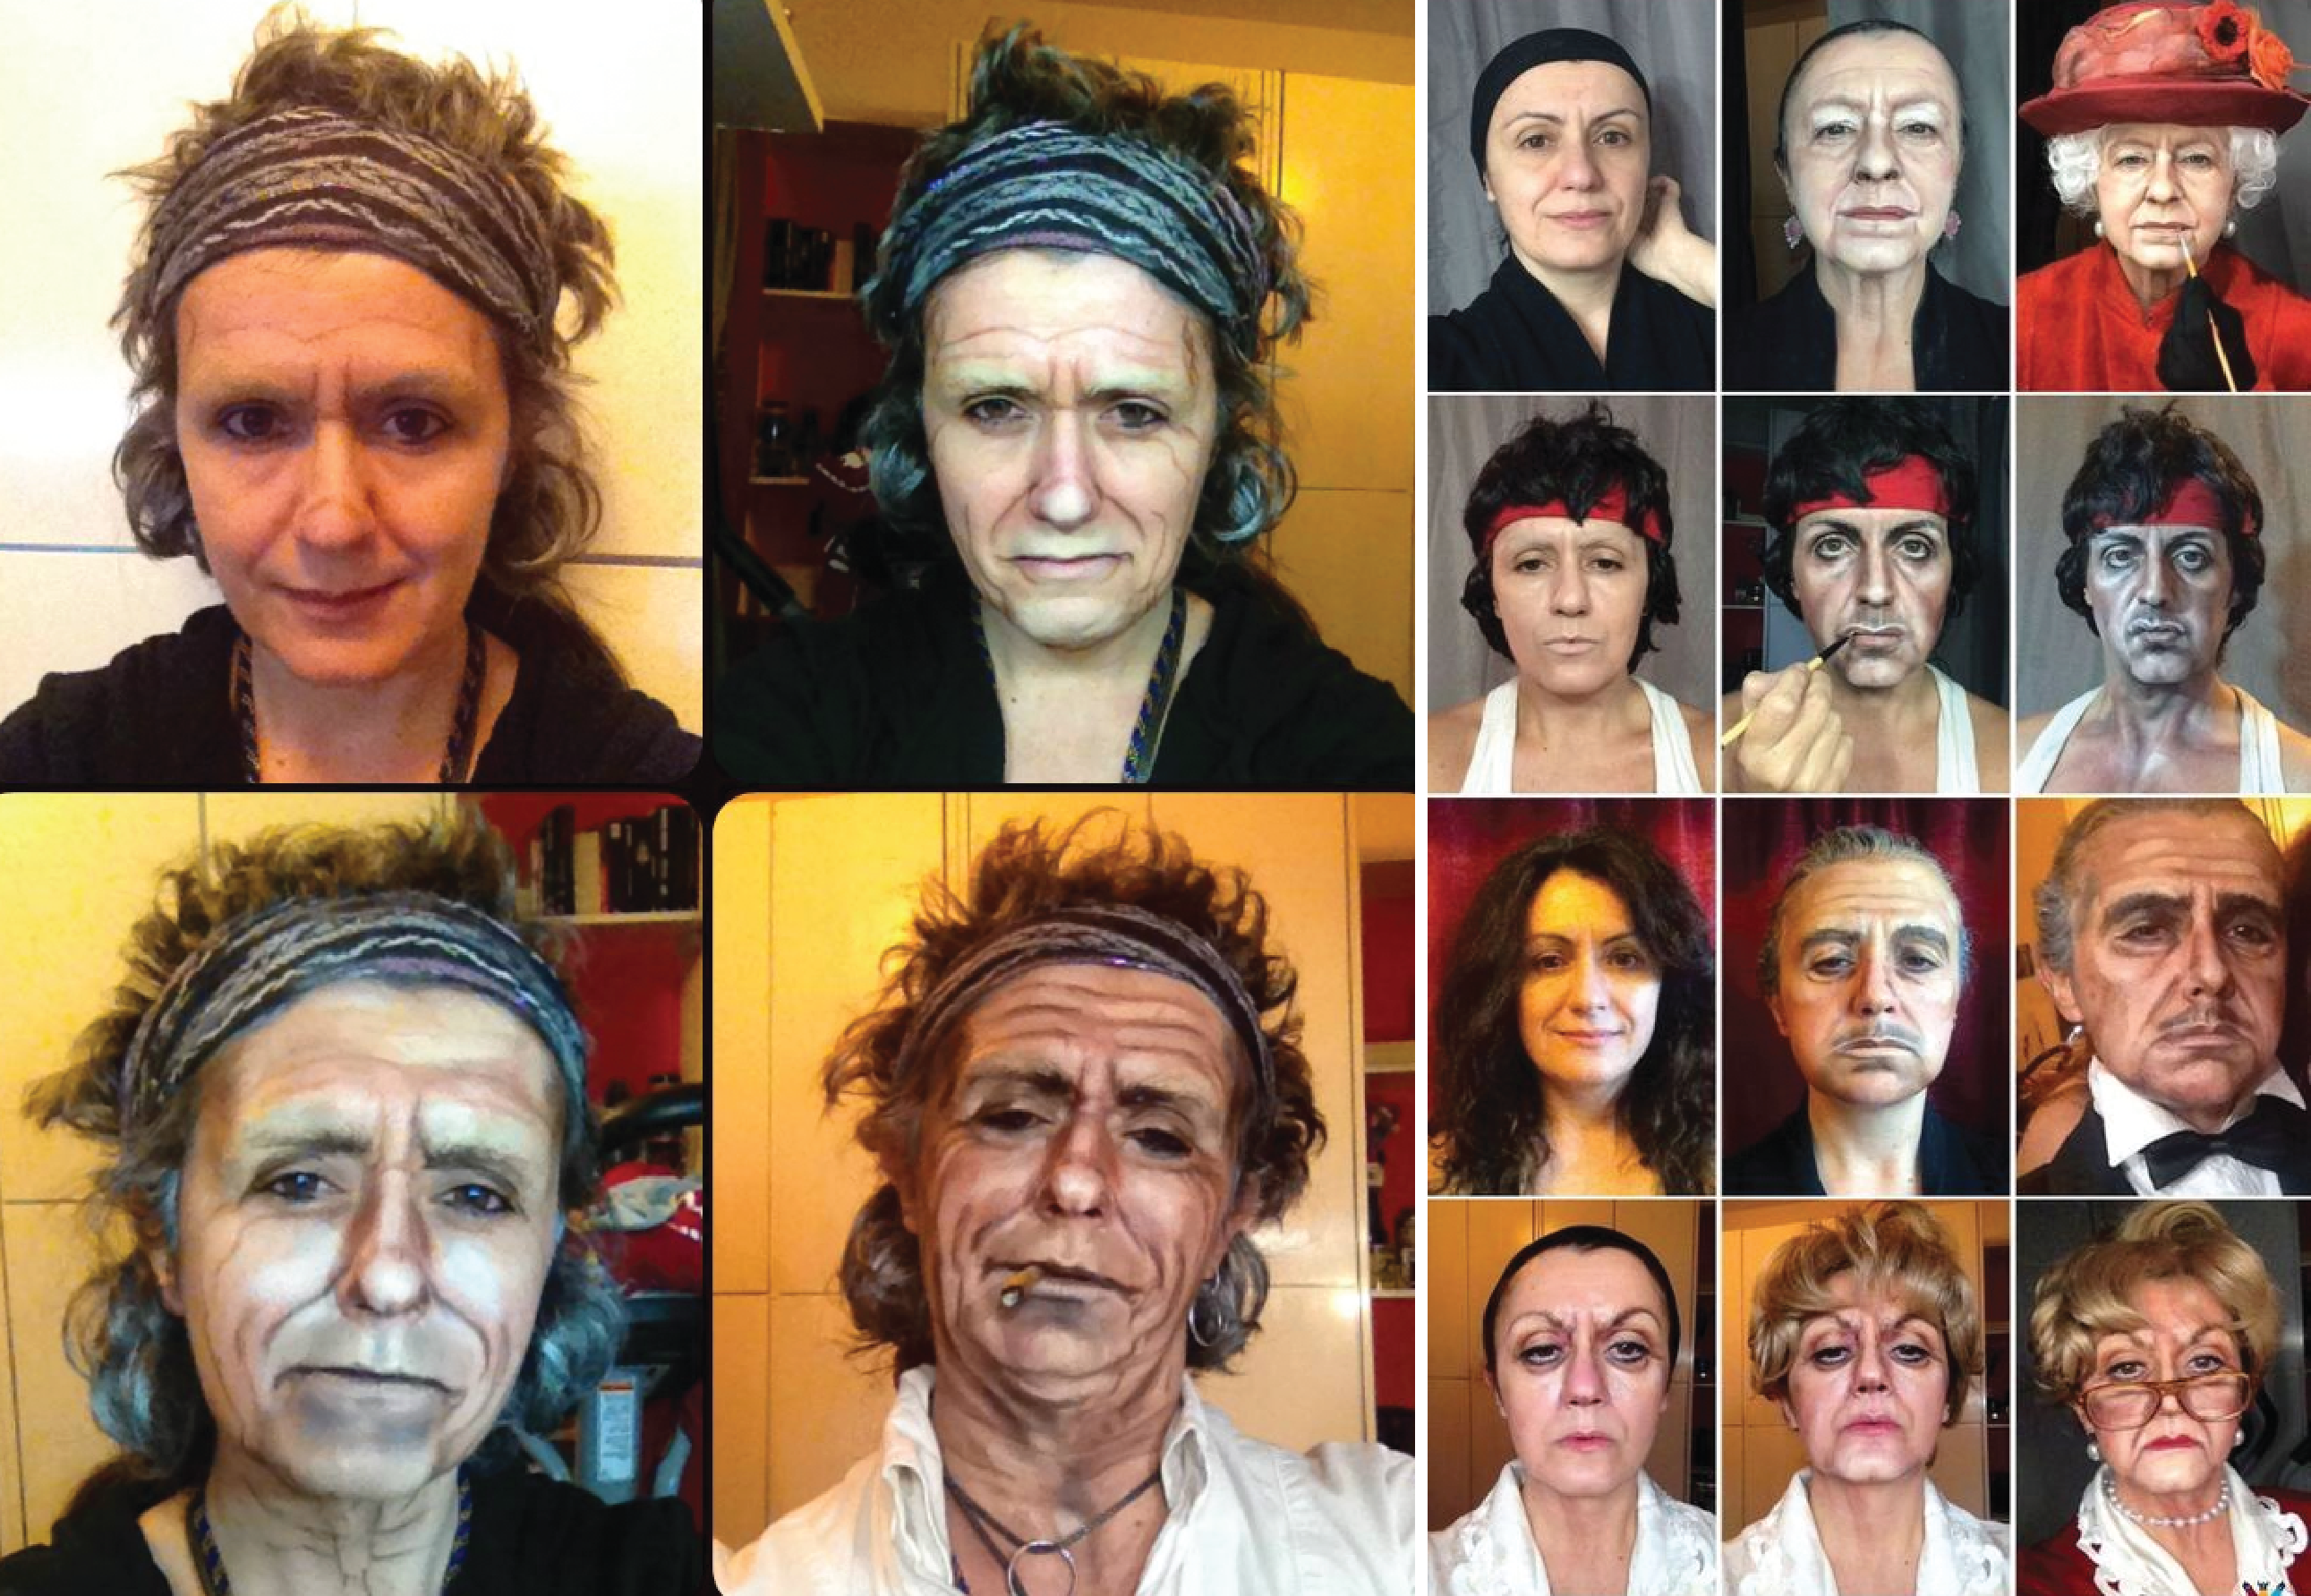
\includegraphics[width=0.8\linewidth]{ch-sistemasABC/images/ch-SistemasABC/MAQUILLADORA_LUCIA_PITTALIS.png}
    \caption{Trabajos de la maquilladora Lucia Pittalis \cite{LuciaPittalisOnline}.}
    \label{fig:Maquillajes}
\end{figure}


Es fácil encontrar distribuidores de mascaras, prótesis y pelucas hiperrealistas que replican perfectamente los rasgos de una persona mediante fotografías (SPFXmask \cite{spfxmaskOnline}, HyperFlesh\cite{HyperFleshOnline}, RealFleshMask \cite{RealFleshMaskhOnline}, ThatsMyFace \cite{ThatsMyFaceOnline}) (ver Fig. \ref{fig:DelitosConMascaras})).

%%%%%%%%%%%%%%%%%%%%%%%%%%%%%%%%%%%  SEGURIDAD_BIOMETRICOS:DETECCION DE ATAQUES DE PRESENTACION %%%%%%%%%%%%%%%%%%%%%%%%%%%%%%%%%%% 
\subsection{Detección de ataques de presentación: PAD}\label{sec:PAD}

Usar biometría en sistemas no supervisados conlleva más riesgos que en sistemas supervisados. Un sistema completamente automático puede ser atacado más fácilmente que uno semiautomático donde alguien controla la adquisición del rasgo biométrico para la identificación. Los \textit{Presentation Attack Detection} (\GLS{PAD}) son las técnicas para detectar automáticamente los ataques de presentación en el momento de la adquisición de las características biométricas del individuo \footnote{\GLS{ISO}/\GLS{IEC} $30107$ describe en detalle muchos de estos métodos de \GLS{PAD} \cite{ISO/PADFramework}.}. Los \GLS{PAD} mitigan los riesgos de ataque y mejoran la seguridad de los sistemas biométricos no supervisados y ayudan en el control en los supervisados.

Es conveniente considerar el \GLS{PAD} como un proceso independiente a la autenticación biométrica y puede realizarse antes o después de ésta. En el mismo dispositivo en el que se realiza la adquisición o bien, mandar los datos capturados o las características a un sistema central. 

Los pasos comunes que deben seguir los métodos de \GLS{PAD} son:

\begin{itemize}
    \item
    Capturar la información biométrica del usuario mediante el sensor o sensores. Estos sensores no tienen por que ser los mismos que los empleados para la adquisición del sistema biométrico, pero es recomendable que la adquisición del \GLS{PAD} se realice de manera simultanea a la del sistema biométrico, con el fin de minimizar los riesgos de seguridad.
    
    \item
    Extracción de las características necesarias para el método \GLS{PAD} especifico. 
    
    \item
    Analizar las características dependiendo del \GLS{PAD} elegido. No hay un método \GLS{PAD} para cada tipo de \GLS{PAI}, un mismo \GLS{PAD} puede detectar distintos tipos de \GLS{PAI}.Y tampoco tiene por que ser el mismo para todos los usuarios, es posible que algunos usuarios requieran un control mas exhaustivo que otros. 
\end{itemize}


%%%%%%%%%%%%%%%%%%%%%%%%%%%%%%%%%%% SEGURIDAD_BIOMETRICOS:TIPOS DE PAD %%%%%%%%%%%%%%%%%%%%%%%%%%%%%%%%%%% 
\subsection{Tipos de PAD}\label{sec:TiposPAD}

Los métodos de \GLS{PAD} pueden ser \textit{hardware} o \textit{software} y dependiendo del nivel del sistema biométrico en el que se implementa el método se puede distinguir entre \GLS{PAD} a nivel sensor o \GLS{PAD} a nivel operacional.

Se pueden clasificar dependiendo de la estrategia que emplean para detectar el ataque.

\paragraph{PAD a nivel sensor:}
\begin{itemize}
    \item 
    \textbf{Detección de artefactos}: Detectan si la presentación está siendo realizada con un objeto sintético.
    
    Ejemplos: Detectar la conductividad de la piel con sensores capacitivos.
    \item 
    \textbf{Detección de vida} \textit{\Gls{liveness detection}}: Son métodos que evalúan las características, o \gls{liveness}, para determinar si realmente hay un individuo con vida frente al dispositivo de adquisición
    
    \Gls{liveness} es la cualidad de vida y se usa en algunos sistemas biométricos para evitar ataques con artefactos o con miembros amputados\footnote{La policía usó el dedo de un cadáver para intentar acceder a su teléfono: \href{https://www.tampabay.com/news/publicsafety/Cops-used-dead-man-s-finger-in-attempt-to-access-his-phone-It-s-legal-but-is-it-okay-\_167262017/}{https://www.tampabay.com/news/publicsafety/Cops-used-dead-man-s-finger-in-attempt-to-access-his-phone-It-s-legal-but-is-it-okay-\_167262017/}} \GLS{PAD} \cite{bhattacharjee2018spoofing} comprueban que el rasgo biométrico se está adquiriendo de una persona viva. Por ejemplos mediante la medición de la temperatura corporal, la detección de los vasos sanguíneos o el parpadeo de los ojos.
    
    Para analizar las reacciones no es suficiente una captura estática se requiere una captura que dure un periodo de tiempo suficiente para que tenga lugar la reacción.
    
    Se pueden considerar $3$ tipos de indicadores que se usan para confirmar una presentación con vida.

    \begin{itemize}
      \item 
      \textbf{Características físicas o anatómicas}: Adsorción de la luz por la piel. Transmisión de electricidad por el cuerpo humano. Transpiración de los dedos. Movimientos del \GLS{iris} o parpadeos. Detección del pulso. Flujo sanguíneo.
      \item
      \textbf{Reacciones involuntarias}: Pulso o dilatación del la pupila al recibir una luz potente.
      \item
      \textbf{Reacciones voluntarias}: Elegir un dedo de la mano. Guiñar un ojo o colocar la mano de una manera determinada.
    \end{itemize}
    
    Algunos métodos para la detección de vida usan estrategias similares a las de reto-respuesta.
    
    \item 
    \textbf{Detección de alteraciones}: Detectar las alteraciones o ocultaciones de un rasgo biométrico.
    
    Ejemplo: Ocultar las huellas dactilares mediante cicatrices. Lentillas sintéticas.
    \item 
    \textbf{Detección de no conformidad}: Detecta conductas extrañas en el usuario al realizar la presentación. 
    
    Ejemplo: No tomar la pose adecuada para la captura \gls{facial} o intentar colocar mal el dedo en el escáner \gls{dactilar}.
    \item 
    \textbf{Detección de coacción}: Detectar si el usuario está siendo coaccionado para realizar realizar la presentación. 
    
    Ejemplos: Detecta rasgos faciales de emociones como el miedo, la angustia, el nerviosismo o el estrés. 
    \item 
    \textbf{Detección de oclusión}: Detecta si el rasgo biométrico o el sensor está siendo ocluido parcial o totalmente. 
    
    Ejemplo: Detectar si el usuario lleva algún complemento que pueda ocluir la captura: Gafas de sol, bufandas, sobreros o guantes. Detectar si algo esta tapando la cámara o el escáner dactilar.
\end{itemize}
    
\paragraph{PAD a nivel operacional:}
\begin{itemize}
    \item 
    \textbf{Limitación de fallos de adquisición}: Contabilizar el número de fallos de adquisición y si se supera un determinado número de fallos la la presentación, considerar lar presentación como un ataque.
    \item
    \textbf{Circunstancias no habituales}: Si la localización o el momento en el que se produce la presentación no es un lugar o un horario habitual, se puede considerar la presentación como un ataque o al menos lanzar una alerta al sistema.  
    \item
    \textbf{Reto-respuesta} (\textit{\gls{challenge response}}): Estrategia que se usa para la autenticación de usuarios que consiste en plantear un reto que requiere una determinada actuación razonada por parte del usuario \cite{shoukry2015pycra}. Normalmente se usa para la autenticación en sistemas no exclusivamente biométricos, donde al usuario se le hace una pregunta o directamente se le solicita una clave.
    
    En los sistemas biométricos la estrategia reto-respuesta se usa como \GLS{PAD} de detección de vida y que los retos plateados pueden ser voluntarios (detección de vida <<activa>>) o involuntarios (detección de vida <<pasiva>>).
    
    \begin{itemize}
        \item
        \textbf{Involuntario}: 
        Un estimulo que provoque una acción determinada, una luz fuerte que provoque una dilatación de la pupila o parpadeos en el usuario \cite{rigas2015eye}.
        \item
        \textbf{Voluntario}:
        Hacer que el usuario dirija su mirada a una determinada región de la pantalla, que guiñe un ojo o que presente al sensor un dedo determinado u otro.
    \end{itemize} 
\end{itemize}

%%%%%%%%%%%%%%%%%%%%%%% ATAQUES DE PRESENTACION Y PAD EN ABC %%%%%%%%%%%%%%%%%%%%%%
\subsection{Ataques de presentación y PAD en sistemas ABC}\label{subsec:PA-biometriasABC}

%%%%%%%%%%%%%%%%%%%%%%% ATAQUES DE PRESENTACION  BIOMETRIA FACIAL %%%%%%%%%%%%%%%%%%%%%%
\paragraph{Ataques de presentación en la biometría facial}
Los ataques de suplantación el la \gls{biometria} \gls{facial} de los sistemas \GLS{ABC} puede producirse de forma directa, mediante un \GLS{PAI} que reproduzca los rasgos faciales del viajero suplantado (Máscaras, maquillaje, etc.) o de forma indirecta, alterando la información biométricas almacenada en el chip del \gls{eMRTD} (\Gls{morphing}).

Los ataques directos pueden ser más o menos detectables por parte de los agentes que monitorizan el sistema. Por ejemplo, una fotografía del viajero o un dispositivos que reproduzca su imagen, pueden engañar al sistema biométrico, pero difícilmente pasarán desapercibidos a los agentes de frontera. Sin embargo, otros \GLS{PAI} como una mascara o prótesis de silicona, o un buen maquillaje  pueden engañar al sistema biométrico y también pueden ser \textbf{indetectables} para los agentes (ver Fig. \ref{fig:DelitosConMascaras}).    


%%%%%%%%%%%%%%%%%%%%%%% ATAQUES DE PRESENTACION BIOMETRIA DACTILAR %%%%%%%%%%%%%%%%%%%%%%
\paragraph{Ataques de presentación en la biometría \gls{dactilar}}
Los ataques a este tipo de biométrica suelen ser \textbf{más discretos} y menos detectables para los agentes de frontera.

Para engañar a los sistemas biométricos dactilares suele usarse como \GLS{PAI} huellas impresas en papel, huellas sintéticas de látex o de gelatina colocadas sobre las huellas reales o incluso dedos amputados del viajero a suplantar. 

Para hacer frente a este tipo de ataques se pueden usar \textbf{métodos \textit{hardware}} con sensores que detectan algunos de estos \GLS{PAI} o \textbf{métodos \textit{software}} que procesan la imagen de la huella dactilar.  

Si se usan \textit{varias huellas} para la identificación, será más difícil atacar al sistema ya que el atacante necesita disponer de más información del viajero a suplantar. Además se puede hacer un control activo de \gls{liveness} solicitando aleatoriamente en la adquisición, una huella u otra.

Detectar el flujo sanguíneo mediante el análisis de las pulsaciones o mediante el análisis de los capilares venosos de la yema de los dedos.

Analizar las condiciones de la piel como la sudoración o el tamaño de algunos rasgos de la huella como los poros

%%%%%%%%%%%%%%%%%%%%%%% ATAQUES DE PRESENTACION BIOMETRIA IRIS %%%%%%%%%%%%%%%%%%%%%%
\paragraph{Ataques de presentación en la biometría del iris}
Suelen usarse lentillas con imágenes del iris del viajero a suplantar o con fotografías de alta resolución.

Para evitar estos ataques es posible analizar las micro-texturas del iris presentado o aplicar métodos de \gls{liveness} como detectar el parpadeo y de \textit{\gls{challenge response}} mediante una luz fuerte que dilate la pupila o haga parpadear al viajero.


%%%%%%%%%%%%%%%%%%%%%%%%%%%%%%%%%%% SEGURIDAD_BIOMETRICOS:EVALUACION DE LOS PAD %%%%%%%%%%%%%%%%%%%%%%%%%%%%%%%%%%% 
\subsection{Evaluación y métricas PAD}\label{sec:MetricasEvaluacionPAD}

Los \GLS{PAD} están sujetos a errores similares a los sistemas biométricos (para más información sobre las métricas de los sistemas biométricos ver Apéndice \ref{apendix:Biometria}), pero por ejemplo \Gls{FAR} no es un buen indicador para medir la vulnerabilidad de un sistema biométrico, ya que informa de cuando un usuario es aceptado como si se tratase de otro pero se esto requiere cero esfuerzo por parte del usuario que sólo hace uso de si propia biometría sin intenciones delictivas.

A partir de $2017$ (\textbf{ISO/IEC $2382$-$37$:$2017$} \cite{ISO/PADEvaluation}), se define una métrica especifica para evaluar la calidad de los sistemas \GLS{PAD}, basada en dos ratios: la tasa de los ataques clasificados de forma errónea, \textit{Attack Presentation Classificacion Error Rate} (\gls{APCER}) y la tasa de las presentaciones del rasgo real \gls{bona-fide} mal clasificadas, \textit{Bona-Fide Presentation Classification Error Rate} (\gls{BPCER}).

\GLS{APCER} y \GLS{BPCER} vienen definidas por las ecuaciones \eqref{eqn:APCER} y \eqref{eqn:BPCER}:

\begin{equation}
APCER_{PAIS} = 1 - \left( \frac{1}{N_{PAIS}} \right)\sum_{i=1}^{N_{PAIS}} \left( RES_{i} \right),
\label{eqn:APCER}
\end{equation}

donde $N_{PAIS}$ es el número de presentaciones de ataque realizados con un determinado \GLS{PAI} (dado que los ataques pueden ser muy diversos, se pueden agrupar según su \GLS{PAI}) y $RES_{i}$ toma el valor $1$ si la presentación \textit{i} es clasificada como ataque y $0$ si es clasificada como \gls{bona-fide}.  

\begin{equation}
BPCER_{PAIS}=\frac{\sum_{i=1}^{N_{BF}} RES_{i}} {N_{BF}},
\label{eqn:BPCER}
\end{equation}

donde $N_{BF}$ es el número de presentaciones \gls{bona-fide} y $RES_{i}$ toma el valor $1$ si la presentación \textit{i} es clasificada como ataque y $0$ si es clasificada como \gls{bona-fide}.  

Habitualmente la respuesta de un sistema \GLS{PAD} es una probabilidad, lo que hace que los valores \GLS{APCER} y \GLS{BPCER} dependan de un umbral con el que se decide si la presentación es un ataque o un \gls{bona-fide}, si la probabilidad es menor o mayor al umbral. 


\begin{figure}
    \centering
    \includegraphics[width=0.8\textwidth]{ch-sistemasABC/images/ch-SistemasABC/EJEMPLO_CURVA_DET_APCER_BPCER.png}
    \caption{Ejemplo de curva \GLS{DET} con el \GLS{APCER} y el \GLS{BPCER} de dos \GLS{PAD}, donde PAD-B es más vulnerable que PAD-A.}
    \label{fig:ejemploCurvaAPCER-BPCER}
\end{figure}

% \begin{SCfigure}[]
%     \centering
%     \sidecaptionvpos{figure}{t}
%     \caption{Ejemplo de curva \GlS{DET} con el \GlS{APCER} y el \GSL{BPCER} de dos \GSL{PAD}, donde PAD-B es más vulnerable que PAD-A.}
%     \includegraphics[width=0.5\textwidth]{ch-sistemasABC/images/EJEMPLO_CURVA_DET_APCER_BPCER.png}
%     \label{fig:ejemploCurvaAPCER-BPCER}
% \end{SCfigure}

Trazando una curva \textit{Error Trade-Off} (\GLS{DET}) con los valores \GLS{APCER} y \GLS{BPCER} para los distintos umbrales es posible visualizar el rendimiento del sistema \GLS{PAD} y comparar unos sistemas con otros. Las curvas más cercanas al origen presentan un \GLS{D-EER} más bajo y por lo tanto un mejor rendimiento (ver Fig. \ref{fig:ejemploCurvaAPCER-BPCER}). 

Al igual que en los sistemas biométricos, ambas tasas, \GLS{APCER} y \GLS{BPCER}, no pueden ser minimizados. \GLS{APCER} se considera una medida de la seguridad del sistema, mientras que el \GLS{BPCER} es una medida de la conveniencia del sistema y normalmente la disminución del \GLS{APCER} implica un aumento del \GLS{BPCER}. En los sistemas \GLS{ABC} debe considerarse la seguridad como el factor más importante frente a la conveniencia. Es aconsejable establecer un valor umbral que devuelva un bajo \GLS{APCER} aunque aumente el \GLS{BPCER}. Ya que los sistemas \GLS{ABC} deben estar controlados por un agente, siempre que una presentación \gls{bona-fide} sea considerada como un ataque, disparará una alarma, que puede ser verificada y corregida por un agente

Otra manera de mostrar el rendimiento de un sistemas \GLS{PAD} consiste en presentar el porcentaje de \gls{bona-fide} mal clasificados (\GLS{BPCER}) cuando se fija un porcentaje de ataques clasificados erróneamente (\GLS{APCER}). (p. ej. Porcentaje de \GLS{BPCER} cuando el \GLS{APCER} es un $5$\%).

Una buena forma de determinar un umbral de aceptación es elegir el umbral en el que los valores de \GLS{BPCER} y \GLS{APCER} son iguales. Este valor se conoce \textit{Detection Equal Error Rate} (\GLS{D-EER}) (ver Fig. \ref{fig:ejemploCurvaAPCER-BPCER}).

.


%ESTO ES DEL PAPER DE MORHPING SE PUEDE BORRAR SI NO APORTA MAS DE LO QUE HAY METIDO
% This section presents the evaluation metrics commonly followed in the morphing attacks detection approaches and the results obtained in the presented work.

% \subsection{Evaluation metrics}\label{sec:EvaluationMetrics}

% Recently, the community has achieved a common standard ISO (IEC 30107-3:2016) \cite{ISO/PADEvaluation} to evaluate PAD systems. In this standard, the capability of the attack detection is measured with the following errors: attack presentation classification error rate (APCER) and bona fide presentation classification error rate (BPCER). This measure can be defined as follows:

% \begin{itemize}
%     \item \textbf{Attack presentation classification error rate (APCER)} is defined as the proportion of presentation attacks that have been classified incorrectly (as bona fide) \cite{ISO/PADEvaluation} (Equation \ref{eqn:APCER}).
%     \item \textbf{Bona fide presentation classification error rate (BPCER)}  is defined as the proportion of bona fide presentation incorrectly classified as presentation attacks \cite{ISO/PADEvaluation} (Equation \ref{eqn:BPCER}).
% \end{itemize}

% \begin{equation}
% APCER_{PAIs} = 1 - \left( \frac{1}{|PAI|} \right)\sum_{\omega=1}^{|PAI|} \left( RES_{\omega} \right),
% \label{eqn:APCER}
% \end{equation}

% where $|PAI|$ is the number of presentation attack instruments (PAI) and $RES_{\omega}$ takes the value $1$ if the presentation $\omega$ is assessed as attack and $0$ if it is evaluated as bona fide. A PAI is defined as a used object or biometric trait in a presentation attack.

% \begin{equation}
% BPCER_{PAIs}=\frac{\sum_{\omega=1}^{|BF|} RES_{\omega}} {|BF|},
% \label{eqn:BPCER}
% \end{equation}

% where $|BF|$ is the cardinality of bona fide presentations and $RES_{i}$ returns the value $1$ if the presentation \textit{$\omega$} is allocated as an attack and $0$ if it is analyzed as bona fide. 

% An APCER-BPCER DET curve (detection error trade-off) and the EER (equal error rate) where both errors are identical, provides a comparison among MAD systems.
